%
% Capítulo 6
%
\chapter{Backend Implementation} \label{cap:backend_implementation}

The backend application is tasked with handling http requests, business logic and data persistence. 

The backend logic is implemented in C{\#} and data is persisted in a postgreSQL database, interaction with this database is done trough EF CORE.

An overview of the backend implementation is presented in Figure ~\ref{fig:backend_implementation}.
\begin{figure}[h]
	\begin{center}
		\resizebox{90mm}{!}{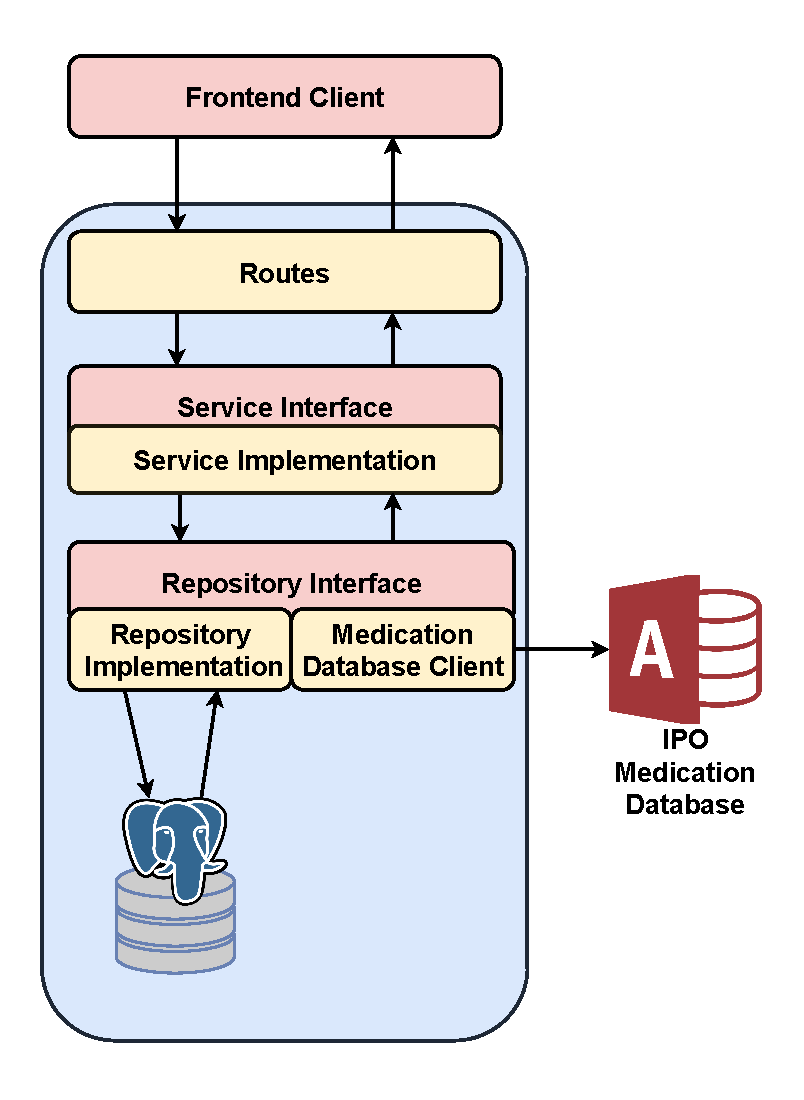
\includegraphics{./figures/backend_implementation.pdf}}
	\end{center}
	\caption{Block Diagram of our solution.}\label{fig:backend_implementation}
\end{figure}

\newpage

\section{Structure}

The structure for the backend application is as follows:

\begin{itemize}
	\item Program.cs: the entry point of the application;
	\item domain: contains all the domain classes;
	\item repositories: contains the backend repositories that communicate with the postgreSQL database;
	\begin{itemize}
		\item entities: contains the entities outlined in chapter \ref{cap:data_model}.
	\end{itemize}
	\item services: contains all the services that, validate and manipulate data, that is received or sent to the routes and repository layer;
	\item routes: contains all the routes of the API which call the adequate service.
	\item utils: contains auxiliary classes and methods.
\end{itemize}

\section{Program.cs}

The .NET framework makes use of a dependency injection container, aka the service container. As with the Spring Framework, dependencies can have various lifetimes, which in the .NET framework are as follows:
\begin{itemize}
	\item Transient: the dependency is created when needed and disposed thereafter;
	\item Scoped: the dependency is created and maintained in a per request basis;
	\item Singleton: once the dependency is created it's maintained throughout the application's lifetime. 
\end{itemize}
Beyond this, the framework also makes use of the builder pattern, meaning to build a web application we first instantiate a builder, i.e. a class that "knows" how to build a web application, and then supply the needed middlewares to build it, with the desired lifetime.
The aforementioned middlewares, which refer to the services and repositories, are registered as services in the container. In our application most of these services were registered with the Scoped scope, as illustrated in Listing \ref{DI}.

\begin{lstlisting}[style=sharpc, caption={Registering Scoped Services in ASP.NET Core Dependency Injection Container.}, label={DI}]
builder.Services.AddScoped<IUsersService, UsersService>();
builder.Services.AddScoped<IFormService, FormService>();
builder.Services.AddScoped<ITermsService, TermsService>();
builder.Services.AddScoped<IMedicationsService, MedicationsService>();
builder.Services.AddScoped<IManualService, ManualService>();
builder.Services.AddScoped<ISubmissionService, SubmissionService>();
builder.Services.AddScoped<IReviewsService, ReviewsService>();

builder.Services.AddScoped<IRepository, Repository>();
\end{lstlisting}

Using this registration method, for example, when a dependency of type IUsersService is needed, the service container creates a UsersService object to fufill that dependency, hence the inversion of control.

The services that don't make use of the scoped lifetime are associated with the lock management and server sent events, are illustrated in \ref{SSE_listing}, these services are elaborated on section \ref{label}.

\begin{lstlisting}[style=sharpc, caption={Registering Scoped Services in ASP.NET Core Dependency Injection Container:}, label={SSE_listing}]
builder.Services.AddSingleton<INotificationService, NotificationService>();
builder.Services.AddSingleton<NotificationEndpoint>();
builder.Services.AddHostedService<UnlockExpiredSubmissionsService>();

\end{lstlisting}

To allow for cross-origin resource sharing, i.e. to allow the frontend client to access the resources in the backend, we also had to create CORS policy, as follows:

\begin{lstlisting}[style=sharpc, caption={Configuring CORS Policy in ASP.NET Core: Allowing Specific Origin with Full Access Control.}]
builder.Services.AddCors(options =>
{
	options.AddPolicy("MyCorsPolicy",
	policy =>
	{
		policy.WithOrigins("http://localhost:8000")
		.AllowAnyHeader()
		.AllowAnyMethod()
		.AllowCredentials();
	});
});
\end{lstlisting}

Notice that request originating from port 8000 of the localhost ip can have any type of header, any HTTP method and can include credentials, such as cookies.
\newpage

\subsubsection{Authentication JWT}

Our platform uses JSON Web Tokens, \textbf{JWT} \cite{rfc7519}, to represent user claims.
These token's issuer, audience and key, refered to as jwtIssuer, jwtAudience and jwtKey in listing \ref{authentication} below, are stored in the appsettings.json file.

\begin{lstlisting}[style=sharpc, caption={Custom JWT Authentication Middleware in ASP.NET Core: Handling Unauthorized Access with Detailed Problem Responses.}, label={authentication}] 
builder.Services.AddAuthentication(x =>
{
	x.DefaultAuthenticateScheme = JwtBearerDefaults.AuthenticationScheme;
	x.DefaultChallengeScheme = JwtBearerDefaults.AuthenticationScheme;
}).AddJwtBearer(options =>
{
	options.Events = new JwtBearerEvents
	{
		...
		OnChallenge = context =>
		{
			context.HandleResponse();
			
			context.Response.ContentType = "application/problem+json";
			context.Response.StatusCode = StatusCodes.Status401Unauthorized;
			var problemDetails = new
			{
				type = "https://localhost:8000/errors/unauthorized",
				title = "Unauthorized",
				detail = "You are not authorized to access this resource. Please provide valid credentials.",
				status = StatusCodes.Status401Unauthorized
			};
			var problemJson = JsonSerializer.Serialize(problemDetails);
			return context.Response.WriteAsync(problemJson);
		}
	};
	options.SaveToken = true;
	options.TokenValidationParameters = new TokenValidationParameters
	{
		ValidateIssuer = true,
		ValidateAudience = true,
		ValidateLifetime = true,
		ValidateIssuerSigningKey = true,
		ValidIssuer = jwtIssuer,
		ValidAudience = jwtAudience,
		IssuerSigningKey = new SymmetricSecurityKey(Encoding.UTF8.GetBytes(jwtKey))
	};
});
\end{lstlisting}

Notice that in case the \textbf{JWT} isn't valid the default behavior of responding with a 401 status code and an empty body is suppressed by "context.HandleResponse()" and instead a Problem response is sent with more details.

\subsubsection{Role Based Access Control}
In our system, users are assigned one of three roles: donor, doctor, or admin. Each of these roles grants access to a specific set of endpoints, ensuring that users can only interact with the parts of the application that are relevant to their role. To enforce this, we have configured authorization policies within the ASP.NET Core framework, which restrict access based on the role claims present in the user's JSON Web Token (JWT).

As shown in Listing \ref{rbac}, we define three authorization policies—one for each role. The AddAuthorization method is used to add these policies to the service container. Each policy requires that the user’s JWT contains a claim of type ClaimTypes.Role with a corresponding value of either donor, doctor", or admin.

\begin{lstlisting}[style=sharpc, caption={Configuring Role-Based Authorization Policies in ASP.NET Core: Defining Access Control for Donor, Doctor, and Admin Roles.}, label={rbac}] 
builder.Services.AddAuthorization(options =>
{
	options.AddPolicy("donor", policy => policy.RequireClaim(ClaimTypes.Role, "donor"));
	options.AddPolicy("doctor", policy => policy.RequireClaim(ClaimTypes.Role, "doctor"));
	options.AddPolicy("admin", policy => policy.RequireClaim(ClaimTypes.Role, "admin"));
});
\end{lstlisting}

When defining an endpoint, we can specify which authorization policy should be applied. For instance, an endpoint that should only be accessible to doctors can be protected by the "doctor" policy.

By leveraging these role-based authorization policies, we enforce a clear and secure access control mechanism, ensuring that users can only perform actions that are appropriate for their role. This approach not only enhances security but also simplifies the management of user permissions across the application.

%Beyond these, we also used an ElasticClient, however in this service registration, we use a different pattern, instead of using a type and implementation, only the latter was used, this method doesn't allow for multiple implementation, but since there was no need to mock the elastic search database, this feature wasn't needed.
%
%\begin{lstlisting}[style=sharpc]
%var nodePool = new SingleNodePool(new Uri("http://localhost:9200"));
%var settings = new ElasticsearchClientSettings(
% nodePool,
% sourceSerializer: (_, settings) =>
%  {
	%    return new DefaultSourceSerializer(settings, options =>
	%      {
		%        options.Converters.Add(new AnswerConverter());
		%        options.Converters.Add(new ConditionConverter());
		%      });
	%  });
%builder.Services.AddSingleton(new ElasticsearchClient(settings));
%\end{lstlisting}
%
%According to the Elastic Search documentation, as long as the client instance is a singleton, our application database is thread safe.
\newpage
\subsection{Repositories}

The Repository layer acts as a vital intermediary for data access within the application. It ensures the database and service layer remain independent from one another. This separation allows the service layer to access data without being tightly coupled to the database, facilitating easy database switching by merely replacing this module.

By defining a well-known interface contract, we can abstract the implementation details.

Utilizing a transaction manager in the service layer enables our solution to handle multiple concurrent accesses across various resources and provides rollback capabilities for effective error handling.

%The main idea in the repositories is to allow for CRUD operations, ie create users/forms, read users/forms, update users/forms and delete users/forms, on data that is or will be stored in an Elastic Search database. As such the repositories have a dependency on the ElasticsearchClient mentioned before, and they'll use the same client but target different indexes.

\subsubsection{Form Repository}

The form repository is responsible for the Form, Submission, Review, Inconsistency entities.

And this repository will have the following methods:

\begin{lstlisting}[style=sharpc]
	public interface IFormRepository
	{
		public Task<Form> GetForm();
		
		public Task<Form?> GetFormWithVersion(int version);
		
		public Task<Form> EditForm(Form form);
		
		public Task<bool> SubmitForm(Submission submission);
		
		public Task<List<Submission>?> GetPendingSubmissions();
		
		public Task<Submission> GetSubmission(int nic);
		
		public Task<Submission?> GetSubmissionById(int id);
		
		public Task<Submission?> GetLatestPendingSubmissionByUser(int userNic);
		
		public Task<(List<SubmissionHistoryDto>? Submissions, bool HasMoreSubmissions)> GetSubmissionHistoryByNic(int nic, int limit, int skip);
		
		public Task<Inconsistencies> GetInconsistencies();
		
		public Task<bool> LockSubmission(int submissionId, int doctorId);
		
		public Task<bool> UnlockSubmission(int submissionId, int doctorId);
		
		public Task<List<SubmissionLock>> GetExpiredLocks(TimeSpan timeout);
		
		public Task<bool> SubmissionExists(int id);
		
		public Task<Review> AddReview(Review review);
		
		public Task<bool> AddNote(Note note);
		
		public Task<bool> EditInconsistencies(Inconsistencies inconsistencies);
	}
\end{lstlisting}

\subsubsection{User Repository}

The user repository will be responsible for the User, UserAccountStatus and UserSuspension entities

And this repository will have the following methods:
\begin{lstlisting}[style=sharpc]
	public interface IUsersRepository
	{
		public Task<bool> AddUser(User user);
		
		public Task<List<User>?> GetUsers();
		
		public Task<User?> GetUserByNic(int nic);
		
		public Task<Boolean> DeleteUser(int nic);
		
		public Task<UserAccountStatus?> GetUserAccountStatus(int userNic);
		
		public Task<Boolean> UpdateUserAccountStatus(UserAccountStatus userAccountStatus);
		
		public Task<bool> AddSuspension(UserSuspension suspension);
		public Task<bool> UpdateSuspension(UserSuspension suspension);
		public Task<UserSuspension?> GetSuspension(int userNic);
		public Task<bool> DeleteSuspension(int userNic);
		
	}
\end{lstlisting}

\newpage

\subsection{Services}
Each service is responsible for managing a certain group of requests, i.e. the logic to fulfill a request to the /users endpoint will be in the user services. Each service as a dependency on their corresponding repository, which is handled by the service container.

The methods within each service will reflect the possible actions outlined in Chapter ~\ref{cap:problem_description}'s section on uses cases.

\subsubsection{Error Handling Implementation}
As mentioned in section \ref{service_layer_error_handling} we will utilize a \textbf{Result} class which can encapsulate either a successful outcome or an error.

To enforce this practice, every service method returns a Result, and each service call in the route layer is wrapped by a HandleRequest method. This method belongs to the HttpExtensions class, as illustrated in Listing \ref{HttpExtensions}.

\begin{lstlisting}[style=sharpc, caption={Custom Extension Methods for Handling HTTP Requests in ASP.NET Core: Simplifying Success and Error Response Handling.}, label={HttpExtensions}]
public static class HttpExtensions
{
	public static IResult HandleRequest<TIn>(
	this Result<TIn> result, Func<TIn,IResult> onSuccess)
	{
		return result.IsSuccess ? onSuccess(result.Value) : Results.Problem(ErrorToProblem(result.Errors[0]));
	}
	
	public static IResult HandleRequest(
	this Result result, Func<IResult> onSuccess)
	{
		return result.IsSuccess ? onSuccess() : Results.Problem(ErrorToProblem(result.Errors[0]));
	}
	
	private static ProblemDetails ErrorToProblem(IError error)
	{
		Console.Out.WriteLine("Error:" + error);
		return new ProblemDetails();
	}
}
\end{lstlisting}


The HandleRequest method is an extension method designed to streamline the handling of HTTP requests by automatically processing the result of a service call.

The first HandleRequest method, defined on lines 3-7, handles cases where the service call returns a value. If the operation is successful (IsSuccess is true), it invokes the onSuccess function, passing the successful result value (result.Value) to generate the appropriate HTTP response. If the operation fails, it calls the Results.Problem method to generate a standardized error response, using the first error in the Errors collection to populate the ProblemDetails object.

Similarly, the second HandleRequest method, defined on lines 9-13, handles cases where the service method returns a Result without a value. It follows the same logic: if the operation is successful, it executes the onSuccess function to produce the HTTP response; otherwise, it generates a ProblemDetails response to represent the error.

The private ErrorToProblem method (lines 15-19) converts an IError object into a ProblemDetails object. This method is responsible for translating internal error details into a standardized format that can be returned as part of an HTTP problem response. The method currently includes a line to output the error details to the console for debugging purposes.

By employing these extension methods, we simplify the process of handling success and error scenarios across the entire application. This ensures that all HTTP responses are consistent, well-structured, and easy to manage, which enhances both the maintainability and reliability of the codebase.

\subsubsection{User Service}

\begin{lstlisting}[style=sharpc]
	public interface IUsersService
	{
		public Task<Result<Token, Problem>> CreateToken(int nic, string password);
		
		public Task<Result<UserExternalInfo, Problem>> CreateUser(int nic, string name, string password, Role role);
		
		public Task<Result<List<UserExternalInfo>, Problem>> GetUsers(string token);
		
		public Task<Result<Boolean, Problem>> DeleteUser(int nic);
		
		public Task<Result<UserAccountStatus?, Problem>> GetUserAccountStatus(int userNic);
		
		public Task<Result<Boolean, Problem>> UpdateUserAccountStatus(UserAccountStatus userAccountStatus);
		
		public Task<Result<UserWithNameExternalInfo?, Problem>> CheckNicExistence(int nic);
		
		public Task<Result<bool, Problem>> AddSuspension(UserSuspensionRequest suspension);
		
		public Task<Result<bool, Problem>> UpdateSuspension(UserSuspension suspension);
		
		public Task<Result<UserSuspension?, Problem>> GetSuspension(int userNic);
		
		public Task<Result<bool, Problem>> DeleteSuspension(int userNic);
	}
\end{lstlisting}

\newpage

\subsubsection{Terms Service}

\begin{lstlisting}[style=sharpc]
	public interface ITermsService
	{
		public Task<Result<List<Terms>, Problem>> GetTerms();
		public Task<Result<Terms, Problem>> GetActiveTerms();
		public Task<Result<bool, Problem>> SubmitTerms(Terms terms);
		
		public Task<Result<bool, Problem>> UpdateTerms(int termId, int updatedBy, string newContent);
		
		public Task<Result<List<TermsChangeLog>?, Problem>> GetTermsChangeLog(int termId);
	}
\end{lstlisting}


\subsubsection{Form Service}

\begin{lstlisting}[style=sharpc]
	public interface IFormService
	{
		public Task<Result<GetFormOutputModel, Problem>> GetForm();
		
		public Task<Result<GetFormWithVersionOutputModel, Problem>> GetFormWithVersion(int version);
		
		public Task<Result<Form, Problem>> EditForm(List<QuestionGroupModel> groups, List<RuleModel> rules, User user);
		
		public Task<Result<SubmitFormOutputModel, Problem>> SubmitForm(Dictionary<string,IAnswer> answers, int nic, int formVersion);
		
		public Task<Result<Submission, Problem>> GetSubmission(int id);
		
		public Task<Result<bool, Problem>> LockSubmission(int submissionId, int doctorId);
		
		public Task<Result<bool, Problem>> UnlockSubmission(int submissionId, int doctorId);
		
		public Task UnlockExpiredSubmissions(TimeSpan lockTimeout);
		
		public Task<Result<Review, Problem>> ReviewForm(int submissionId, int doctorNic, string status, string? finalNote, List<NoteModel>? noteModels = null);
		
		public Task<Result<List<Submission>, Problem>> GetPendingSubmissions();
		
		public Task<Result<Inconsistencies, Problem>> GetInconsistencies();
		
		public Task<Result<Submission?, Problem>> GetPendingSubmissionsByUserNic(int userNic);
		
		public Task<Result<SubmissionHistoryOutputModel, Problem>> GetSubmissionHistoryByNic(int nic, int limit, int skip);
		
		public Task<Result<bool, Problem>> EditInconsistencies(Inconsistencies inconsistencies);
	}
\end{lstlisting}


\subsubsection{Manual Service}

\begin{lstlisting}[style=sharpc]
	public interface IManualService
	{
		public Task<Result<List<ManualInformation>, Problem>> GetManualInformation(string productName);
	}
\end{lstlisting}


\subsubsection{Medication Service}

\begin{lstlisting}[style=sharpc]
	public interface IMedicationsService
	{
		Task<Result<List<string>, Problem>> SearchMedications(string query);
	}
\end{lstlisting}

\newpage

\subsection{Routes}

\subsubsection{User Routes}
The available endpoints, HTTP method and corresponding operation for all the user routes are available in Table ~\ref{tab:user_endpoints}. 

\begin{table}[h!]
	\begin{center}
		\begin{tabular}{l|c|l} 
			\textbf{Endpoint} & \textbf{HTTP Method} & \textbf{Description} \\
			\hline
			/users & POST & \makecell{Creates a new user} \\
			\hline
			/users & GET & \makecell{Retrieves all users} \\
			\hline
			/users/\{nic\} & GET & \makecell{Checks the existence of a user with the specified NIC}\\
			\hline
			/users/\{nic\} & DELETE & \makecell{Deletes the user with the specified NIC} \\
			\hline
			/users/login & POST & \makecell{Creates a new access token} \\
			\hline
			/users/status/\{nic\} & GET & \makecell{Retrieves the status of the user account\\ with the specified NIC} \\
			\hline
			/update-status & POST & \makecell{Updates the status of a user account} \\
			\hline
			/users/suspension & POST & \makecell{Adds a new suspension} \\
			\hline
			/users/suspension/update & POST & \makecell{Updates an existing suspension} \\
			\hline
			/users/suspension/\{nic\} & GET & \makecell{Retrieves the suspension details for the specified NIC} \\
			\hline
			/users/suspension/\{nic\} & DELETE & \makecell{Deletes the suspension for the specified NIC} \\
		\end{tabular}
		
		\caption{API endpoints related to the user}\label{tab:user_endpoints}
	\end{center}
\end{table}

\subsubsection{Form Routes}
The available endpoints, HTTP method and corresponding operation for all the form routes are available in Table ~\ref{tab:form_endpoints}. 

\begin{table}[h!]
	\begin{center}
		\begin{tabular}{l|c|l} 
			\textbf{Endpoint} & \textbf{HTTP Method} & \textbf{Description} \\
			\hline
			/forms/structure & GET & \makecell{Retrieves the form structure} \\
			\hline
			/forms/structure & PUT & \makecell{Edits the form structure} \\
			\hline
			/forms/structure/\{version:int\} & GET & \makecell{Retrieves the form structure \\ for the specified version} \\
			\hline
			/forms/submissions & GET & \makecell{Retrieves pending submissions} \\
			\hline
			/forms/submissions/\{nic:int\} & POST & \makecell{Submits a form} \\
			\hline
			/forms/submissions/\{nic:int\} & GET & \makecell{Retrieves a pending submission \\ for the specified NIC} \\
			\hline
			/forms/submissions/history/\{nic:int\} & GET & \makecell{Retrieves submission history \\ for the specified NIC} \\
			\hline
			/forms/submissions/\{submissionId:int\}/lock & POST & \makecell{Locks a submission} \\
			\hline
			/forms/submissions/\{submissionId:int\}/unlock & POST & \makecell{Unlocks a submission} \\
			\hline
			/forms/inconsistencies & GET & \makecell{Retrieves inconsistencies} \\
			\hline
			/forms/inconsistencies & PUT & \makecell{Edits inconsistencies} \\
			\hline
			/forms/review/\{submissionId:int\} & POST & \makecell{Reviews a form submission} \\
			\hline
			/forms/notifications & GET & \makecell{Sets up server-sent \\ event notifications} \\
		\end{tabular}
		
		\caption{API endpoints related to the form}\label{tab:form_endpoints}
	\end{center}
\end{table}

\subsubsection{Terms Routes}
\begin{table}[h!]
	\begin{center}
		\begin{tabular}{l|c|l} 
			\textbf{Endpoint} & \textbf{HTTP Method} & \textbf{Description} \\
			\hline
			/terms & GET & \makecell{Retrieves all the terms} \\
			\hline
			/terms/active & GET & \makecell{Retrieves the active terms} \\
			\hline
			/terms & POST & \makecell{Submits terms} \\
			\hline
			/terms/\{termsId:int\} & PUT & \makecell{Updates terms with the specified termsId} \\
			\hline
			/terms/change-log/\{termsId:int\} & GET & \makecell{Gets the change-logs\\ for the terms with  specified termsId} \\
		\end{tabular}
		
		\caption{API endpoints related to the form}\label{tab:term_endpoints}
	\end{center}
\end{table}

\subsubsection{Medication and Manual Routes}
\begin{table}[h!]
	\begin{center}
		\begin{tabular}{l|c|l} 
			\textbf{Endpoint} & \textbf{HTTP Method} & \textbf{Description} \\
			\hline
			/medications/search & GET & \makecell{Retrieves medication list according to a query string} \\
			\hline
			/manual/\{product:string\} & GET & \makecell{Retrieves the blood donation information relevant to the specific product} \\
		\end{tabular}
		
		\caption{API endpoints related to the form}\label{tab:medication_manual_endpoints}
	\end{center}
\end{table}

\section{Password Security}\label{sec:security}

Two common password attacks are brute force attacks, and side-channel attacks.

Brute force attacks leverage the high computational power of Graphics Processing Units (GPUs) to paralelize password hashing tasks.

Side-channel attacks try get indirect information leaked during the execution of cryptographic algorithms, ie the time or power it takes for a system to hash a password.

\subsection{Mitigation}

Password hashing is a crucial security measure used to protect stored passwords. Instead of saving passwords in plaintext, which can be easily compromised, passwords are transformed into a hashed format using a hashing algorithm.

The work factor is the number of iterations of the hashing algorithm that are performed for each password. The work factor is typically stored in the hash output. It makes calculating the hash more computationally expensive, which in turn reduces the speed and/or increases the cost for which an attacker can attempt to crack the password hash \cite{owasp_password_storage}, which increases the brute-force attack further.
Choosing a work factor requires a compromise between security and performance, since, if to much computing power is required to hash a password the system becomes targetable to denial of service attacks.

Hashing algorithms that employ constant time operations and parallelism whenever possible help mitigate the risk of side channel attacks, as these factors increases the difficulty to extract information form side-channels.  


\subsection{Argon2id}
Argon2\cite{rfc9106} is a state-of-the-art password hashing algorithm that won the Password Hashing Competition in 2015. It comes in three variants: Argon2d, Argon2i, and Argon2id. Argon2id is a hybrid version that combines the benefits of both Argon2d (which provides resistance against brute-force attacks) and Argon2i (which is designed for side-channel attack resistance), and will be the algorithm used to secure the passwords for our platform.

Argon2id takes in configurable parameter, such as:
\begin{itemize}
	\item \textbf{Memory Cost}: The amount of memory (in kilobytes) used by the algorithm;
	\item \textbf{Time Cost} : The number of iterations the algorithm runs, which affects the computation time;
	\item \textbf{Parallelism} : The number of parallel threads used to process the hash.
\end{itemize}

Since these parameters are configurable it is possible to adjust them throughout the lifetime of an application, for example increase the time cost as the hosting hardware's capacity increases, and decrease it if concurrent accesses increase.

\newpage

\section{Testing}

Testing is a crucial step in ensuring the reliability and functionality of our application. This chapter outlines the approaches and tools used to validate the correctness of our code.

\subsection{Manual Testing}

During the development of the application, particularly on the backend, manual testing was employed to verify that the system behaved as expected. The primary tools used for manual testing were:

\begin{itemize} 
	\item \textbf{Swagger:} Swagger was utilized to test the API through HTTP requests. Although Swagger is primarily an API documentation and automation tool, it provides the necessary features for effective manual testing of APIs. 
	\item \textbf{Postman:} Postman was occasionally used to interact with ElasticSearch, specifically for data retrieval and storage operations. 
\end{itemize}

\subsection{Programmatic Testing}
Programmatic testing involves the use of specialized software tools to ensure the correctness and robustness of the application. This approach allows for repetitive and comprehensive testing of the codebase, improving efficiency and coverage.

\subsubsection{Unit Tests}
Unit tests are designed to verify the behavior of individual components or modules in isolation. We followed the Arrange-Act-Assert (AAA) pattern to structure our unit tests:

\begin{itemize} 
	\item \textbf{Arrange:} Prepare the necessary preconditions and inputs for the test. 
	\item \textbf{Act:} Execute the operation or function being tested. 
	\item \textbf{Assert:} Verify that the outcome matches the expected result. 
\end{itemize}

We employed xUnit.net, a free and open-source unit testing tool for the .NET framework, to execute our unit tests.

\subsubsection{Integration Tests}

TODO
